\chapter{Preliminary for Quantum Computation}\label{ch:sec01}

We begin with the four postulates of quantum mechanics most relevant to quantum
computation; see Nielsen and Chuang for more details. All four postulates
concern \emph{closed} quantum systems, that is, systems isolated from their
environments. \emph{Open} quantum systems, which interact with an environment
and are characterized by a decoherence time, are not treated here.

The four postulates are:
\begin{enumerate}
  \item State space;
  \item Quantum operator;
  \item Quantum measurement;
  \item Tensor product.
\end{enumerate}

\section{State-space postulate}\label{sec:sec01-state-space}

\begin{definition}[State space]
The set of all quantum states of a quantum system forms a complex vector space
with an inner-product structure, i.e.\ a Hilbert space, denoted $\Hilb$.
\end{definition}

For a finite-dimensional state space we have $\Hilb \cong \C^N$ (isomorphic to),
and without loss of generality we take $\Hilb = \C^N$. Throughout we assume
$N = 2^n$, where $n$ is a non-negative integer equal to the number of bits or
qubits.

A quantum state $\psi \in \C^N$ can be expressed as a column vector, together
with its Hermitian conjugate,
\begin{equation}
  \psi = \begin{pmatrix} \psi_0 \\ \psi_1 \\ \vdots \\ \psi_{N-1} \end{pmatrix},
  \qquad
  \psi\dg = \begin{pmatrix} \bar{\psi}_0 & \bar{\psi}_1 & \cdots & \bar{\psi}_{N-1} \end{pmatrix}.
\end{equation}

\paragraph{Dirac notation.}
$\ket{\psi}$ denotes a quantum state $\psi$, and $\bra{\psi}$ denotes its
Hermitian conjugate $\psi\dg$. The inner product is
\begin{equation}
  \braket{\psi|\varphi} := \langle \psi, \varphi \rangle
  = \sum_{i \in [N]} \bar{\psi}_i \varphi_i,
  \qquad [N] = \{0, 1, \dots, N-1\}.
\end{equation}
Let $\{\ket{i}\}$ be the standard basis of $\C^N$. The $i$-th entry of $\psi$ can
be written as $\psi_i = \braket{i|\psi}$. The outer product $\ket{\psi}\bra{\varphi}$
has $(i,j)$-th element
\begin{equation}
  \bra{i}\bigl(\ket{\psi}\bra{\varphi}\bigr)\ket{j}
  = \braket{i|\psi}\braket{\varphi|j} = \psi_i \bar{\varphi}_j.
\end{equation}

Two vectors $\ket{\psi}$ and $c\ket{\psi}$, for some $0 \neq c \in \C$, refer to
the same physical state; that is, $c$ has no observable effects. Hence
$\ket{\psi}$ is always assumed to be normalized to a unit vector,
$\braket{\psi|\psi} = 1$ (sometimes $\psi$ denotes an unnormalized state). For a
normalized state vector, $c = \ee^{\ii\theta}$ with $\theta \in [0, 2\pi)$ is a
global phase factor.

\begin{example}[Single-qubit system]
A single qubit corresponds to a state space $\Hilb \cong \C^2$. Define
\begin{equation}
  \ket{0} = \begin{pmatrix} 1 \\ 0 \end{pmatrix}, \qquad
  \ket{1} = \begin{pmatrix} 0 \\ 1 \end{pmatrix}.
\end{equation}
\end{example}

\begin{remark}
The state space of a spin-$\tfrac{1}{2}$ system is isomorphic to $\C^2$, also
called a single-spin system, where $\ket{0}$ and $\ket{1}$ are referred to as the
spin-up and spin-down states. A general state vector $\psi \in \Hilb$ is
\begin{equation}
  \psi = a\ket{0} + b\ket{1} = \begin{pmatrix} a \\ b \end{pmatrix},
  \qquad a, b \in \C,
\end{equation}
with the normalization condition $\abs{a}^2 + \abs{b}^2 = 1$. Therefore
\begin{equation}
  \ket{\psi} = \ee^{\ii\gamma}\!\left( \cos\tfrac{\theta}{2}\ket{0}
    + \ee^{\ii\varphi}\sin\tfrac{\theta}{2}\ket{1} \right),
  \qquad \gamma, \theta, \varphi \in \R.
\end{equation}
Ignoring the global phase $\gamma$,
\begin{equation}
  \ket{\psi} = \cos\tfrac{\theta}{2}\ket{0}
    + \ee^{\ii\varphi}\sin\tfrac{\theta}{2}\ket{1},
  \qquad 0 \le \theta \le \pi, \quad 0 \le \varphi < 2\pi.
\end{equation}
This gives the Bloch-sphere correspondence
$\ket{\psi} \longleftrightarrow
\vec{a} = (\sin\theta\cos\varphi,\ \sin\theta\sin\varphi,\ \cos\theta)^{\mathsf{T}}$.
\end{remark}

\begin{figure}[ht]
  \centering
  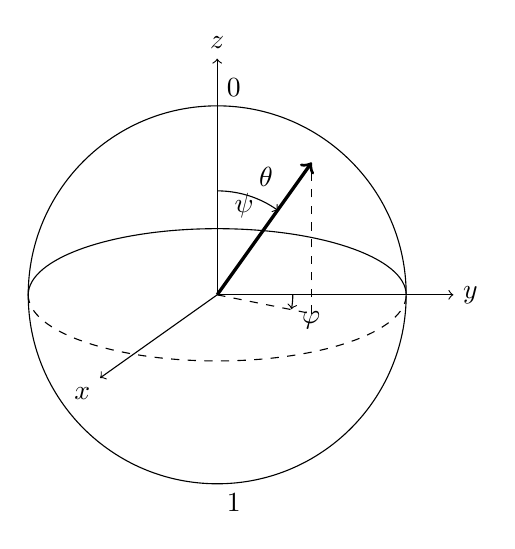
\begin{tikzpicture}[scale=2.4]
    % sphere outline and equator
    \draw (0,0) circle (1);
    \draw[dashed] (-1,0) arc (180:360:1 and 0.35);
    \draw (1,0) arc (0:180:1 and 0.35);
    % axes
    \draw[->] (0,0) -- (0,1.25) node[above] {$z$};
    \draw[->] (0,0) -- (1.25,0) node[right] {$y$};
    \draw[->] (0,0) -- (-0.62,-0.44) node[below left] {$x$};
    % poles
    \node[above right] at (0,1) {$\ket{0}$};
    \node[below right] at (0,-1) {$\ket{1}$};
    % state vector
    \coordinate (O) at (0,0);
    \coordinate (P) at (0.5,0.7);
    \draw[->,very thick] (O) -- (P) node[midway,above left] {$\ket{\psi}$};
    % projection onto equatorial plane
    \coordinate (Q) at (0.5,-0.1);
    \draw[dashed] (O) -- (Q);
    \draw[dashed] (Q) -- (P);
    % polar angle theta (from z axis)
    \draw[->] (0,0.55) arc (90:54:0.55) node[midway,above right] {$\theta$};
    % azimuthal angle phi (in equatorial plane)
    \draw[->] (0.4,0) arc (0:-11:0.4) node[midway,below right] {$\varphi$};
  \end{tikzpicture}
  \caption{Bloch-sphere representation of a single-qubit pure state
    $\ket{\psi} = \cos\tfrac{\theta}{2}\ket{0} + \ee^{\ii\varphi}\sin\tfrac{\theta}{2}\ket{1}$,
    with polar angle $\theta$ and azimuthal angle $\varphi$.}
  \label{fig:sec01-bloch}
\end{figure}

\section{Quantum-operator postulate}\label{sec:sec01-operator}

\begin{definition}[Quantum operator]
The evolution of a quantum state from $\ket{\psi} \to \ket{\psi'} \in \C^N$ is
always achieved via a unitary operator $U \in \C^{N \times N}$, i.e.
\begin{equation}
  \ket{\psi'} = U\ket{\psi}, \qquad U\dg U = I_N.
\end{equation}
\end{definition}

\paragraph{Gate.} In quantum computation, a unitary matrix is often referred to
as a gate.

\begin{example}
For a single qubit, the Pauli matrices are
\begin{equation}
  \sigma_x = X = \begin{pmatrix} 0 & 1 \\ 1 & 0 \end{pmatrix}, \quad
  \sigma_y = Y = \begin{pmatrix} 0 & -\ii \\ \ii & 0 \end{pmatrix}, \quad
  \sigma_z = Z = \begin{pmatrix} 1 & 0 \\ 0 & -1 \end{pmatrix}.
\end{equation}
Some other important single-qubit operators include
\begin{align}
  \text{Hadamard gate} \quad & H = \frac{1}{\sqrt{2}}\begin{pmatrix} 1 & 1 \\ 1 & -1 \end{pmatrix}, \\
  \text{phase gate} \quad & S = \begin{pmatrix} 1 & 0 \\ 0 & \ii \end{pmatrix}, \\
  T \text{ gate} \quad & T = \begin{pmatrix} 1 & 0 \\ 0 & \ee^{\ii\pi/4} \end{pmatrix}.
\end{align}
\end{example}

\paragraph{Clifford and non-Clifford gates.}
The Pauli matrices generate a discrete group, called the Pauli group $\mathcal{P}$.
The Pauli group on $n$ qubits, $\mathcal{P}_n$, is the set of all $n$-qubit tensor
products of elements from $\mathcal{P}$. A \emph{Pauli string} is any element of
$\mathcal{P}_n$ with positive phase. The Clifford group on $n$ qubits,
$\mathcal{C}_n$, is the set of operations which normalize $\mathcal{P}_n$ in the
group-theoretic sense, i.e.\ $U \in \mathcal{C}_n$ if $U P U\dg \in \mathcal{P}_n$
for all $P \in \mathcal{P}_n$. A \emph{Clifford gate} is any unitary in
$\bigcup_{n \ge 1} \mathcal{C}_n$.

A Clifford circuit is a quantum circuit of Clifford gates implementing a unitary
transformation on some set of qubits, designated the input/output qubits, while
preserving the state of the remaining ancilla qubits.

We say a state $\ket{\psi}$ is \emph{stabilized} by an operation $U$ iff
$U\ket{\psi} = \ket{\psi}$. The Pauli elements and the states they stabilize are
as follows:
\begin{align}
  X &: \ket{+} = \tfrac{\ket{0}+\ket{1}}{\sqrt{2}}, &
  -X &: \ket{-} = \tfrac{\ket{0}-\ket{1}}{\sqrt{2}}, \\
  Y &: \ket{\ii} = \tfrac{\ket{0}+\ii\ket{1}}{\sqrt{2}}, &
  -Y &: \ket{-\ii} = \tfrac{\ket{0}-\ii\ket{1}}{\sqrt{2}}, \\
  Z &: \ket{0}, & -Z &: \ket{1}.
\end{align}
\begin{itemize}
  \item Stabilizer gates are composed of CNOT, Hadamard, and $\tfrac{\pi}{4}$-phase
    ($P$) gates, $P = \begin{psmallmatrix} 1 & 0 \\ 0 & \ii \end{psmallmatrix}$.
  \item Stabilizer circuits can be efficiently simulated on classical computers
    (Gottesman--Knill theorem).
\end{itemize}
Any quantum circuit whose computing power exceeds that of classical computers
must employ a non-Clifford gate, such as the $\tfrac{\pi}{8}$-phase or $T$ gate,
$T = \begin{psmallmatrix} 1 & 0 \\ 0 & \ee^{\ii\pi/4} \end{psmallmatrix}$.

\paragraph{$n$-qubit operator.} An operator acting on an $n$-qubit state space
(more details in the quantum-circuits section, \cref{sec:sec01-circuits}).

Starting from an initial quantum state $\ket{\psi(0)}$, it can evolve in time,
which gives a single-parameter family of quantum states $\{\ket{\psi(t)}\}$. The
evolution is determined by a quantum evolution operator $U$:
\begin{equation}
  \psi(t_2) = U(t_2, t_1)\,\psi(t_1),
\end{equation}
where $U(t_2, t_1)$ is unitary for any given $t_2, t_1$. The evolution is
reversible.

\begin{definition}[Schr\"odinger equation]
The quantum evolution under a time-independent Hamiltonian $H$ satisfies the
time-independent Schr\"odinger equation
\begin{equation}
  \ii\,\partial_t \ket{\psi(t)} = H\ket{\psi(t)}.
\end{equation}
\end{definition}

\begin{example}
Let the Hamiltonian $H$ be the Pauli-$X$ gate. Then
\begin{equation}
  U(t, 0) = \ee^{-\ii X t}
  = \begin{pmatrix} \cos t & -\ii\sin t \\ -\ii\sin t & \cos t \end{pmatrix}
  = \cos t\, I - \ii\sin t\, X.
\end{equation}
With $\ket{\psi(0)} = \ket{0}$,
\begin{equation}
  \ket{\psi(\tfrac{\pi}{2})} = \ee^{-\ii\frac{\pi}{2}X}\ket{\psi(0)}
  = -\ii X\ket{0} = -\ii\ket{1}.
\end{equation}
\end{example}

\section{Quantum-measurement postulate}\label{sec:sec01-measurement}

Only projective measurement is discussed here. All quantum measurements
expressed as a positive operator-valued measure (POVM) can be expressed in terms
of projective measurements in an enlarged Hilbert space via the Naimark dilation
theorem.

\begin{definition}[Quantum observable]
In the finite-dimensional setting, a quantum observable corresponds to a
Hermitian matrix $M$, which has the spectral decomposition
\begin{equation}
  M = \sum_m \lambda_m P_m,
\end{equation}
where $\lambda_m \in \R$ is an eigenvalue of $M$ and $P_m$ is the eigen-projection
operator associated with $\lambda_m$, satisfying $P_m^2 = P_m$.
\end{definition}

When a quantum state $\ket{\psi}$ is measured by a quantum observable $M$, the
outcome is an eigenvalue $\lambda_m$, with probability
\begin{equation}
  p_m = \braket{\psi|P_m|\psi}.
\end{equation}
After the measurement, the quantum state becomes
\begin{equation}
  \ket{\psi} \to \frac{P_m\ket{\psi}}{\sqrt{p_m}},
\end{equation}
which is not a unitary process.

\paragraph{Expectation of measurement.}
From the resolution of the identity $\sum_m P_m = I$ it follows that
\begin{equation}
  \sum_m p_m = \sum_m \braket{\psi|P_m|\psi}
  = \bra{\psi}\Bigl(\sum_m P_m\Bigr)\ket{\psi} = \braket{\psi|\psi} = 1,
\end{equation}
and the expected value of $M$ is
\begin{equation}
  \E_\psi(M) = \sum_m \lambda_m p_m
  = \sum_m \lambda_m \braket{\psi|P_m|\psi}
  = \bra{\psi}\Bigl(\sum_m \lambda_m P_m\Bigr)\ket{\psi}
  = \braket{\psi|M|\psi}.
\end{equation}

\begin{example}
Let $M = X = \begin{psmallmatrix} 0 & 1 \\ 1 & 0 \end{psmallmatrix}$, with
$\ket{\pm} := \tfrac{1}{\sqrt{2}}(\ket{0} \pm \ket{1})$ and $\lambda_\pm = \pm 1$.
Then $M = X = \ket{+}\bra{+} - \ket{-}\bra{-}$ and
$\ket{\psi} = \ket{0} = \tfrac{1}{\sqrt{2}}(\ket{+} + \ket{-})$. Hence
$\braket{\psi|P_+|\psi} = \braket{\psi|P_-|\psi} = \tfrac{1}{2}$, so that
$\braket{\psi|M|\psi} = 0$.
\end{example}

\section{Tensor-product postulate}\label{sec:sec01-tensor}

Suppose a quantum state consists of $m$ components with state spaces
$\{\Hilb_i\}_{i=0}^{m-1}$, and let the tensor-product space be
$\Hilb = \bigotimes_{i=0}^{m-1} \Hilb_i$. If $\ket{\psi_i} \in \Hilb_i$, then
$\ket{\psi} = \ket{\psi_0} \otimes \cdots \otimes \ket{\psi_{m-1}} \in \Hilb$.

In general, let $\{\ket{e_j^{(i)}}\}_{j \in [N_i]}$ be a basis of $\Hilb_i$. Then
a general state vector in $\Hilb$ takes the form
\begin{equation}
  \ket{\psi} = \sum_{j_0 \in [N_0], \dots, j_{m-1} \in [N_{m-1}]}
    \psi_{j_0 \cdots j_{m-1}}\,
    \ket{e_{j_0}^{(0)}} \otimes \cdots \otimes \ket{e_{j_{m-1}}^{(m-1)}}.
\end{equation}
Here $\psi_{j_0 \cdots j_{m-1}} \in \C$ is an entry of an $m$-way vector, and
$\dim \Hilb = \prod_{i \in [m]} N_i$.

The $n$-qubit state space is $\Hilb = (\C^2)^{\otimes n} \cong \C^{2^n}$. We also
use the notation
\begin{equation}
  \ket{01} \equiv \ket{0,1} \equiv \ket{0}\ket{1} \equiv \ket{0}\otimes\ket{1},
  \qquad \ket{0^{\otimes n}} = \ket{0}^{\otimes n}.
\end{equation}
For a classical bit-string $x \in \{0,1\}^n$, the set
$\{\ket{x} : x \in \{0,1\}^n\}$ is the computational basis of $\C^{2^n}$.

\begin{example}[Two-qubit system]
The state space is $\Hilb = (\C^2)^{\otimes 2} \cong \C^4$. In the standard basis
(row-major order, i.e.\ the last index is fastest-changing),
\begin{equation}
  \ket{00} = \begin{psmallmatrix} 1 \\ 0 \\ 0 \\ 0 \end{psmallmatrix}, \quad
  \ket{01} = \begin{psmallmatrix} 0 \\ 1 \\ 0 \\ 0 \end{psmallmatrix}, \quad
  \ket{10} = \begin{psmallmatrix} 0 \\ 0 \\ 1 \\ 0 \end{psmallmatrix}, \quad
  \ket{11} = \begin{psmallmatrix} 0 \\ 0 \\ 0 \\ 1 \end{psmallmatrix}.
\end{equation}
The Bell state (EPR pair) is
\begin{equation}
  \ket{\psi} = \tfrac{1}{\sqrt{2}}(\ket{00} + \ket{11})
  = \tfrac{1}{\sqrt{2}}\begin{psmallmatrix} 1 \\ 0 \\ 0 \\ 1 \end{psmallmatrix},
\end{equation}
which cannot be written as any product state $\ket{a} \otimes \ket{b}$; it is
\emph{entangled}.
\end{example}

An important two-qubit quantum operator is the CNOT gate (controlled-NOT),
\begin{equation}
  \mathrm{CNOT} = \begin{pmatrix}
    1 & 0 & 0 & 0 \\
    0 & 1 & 0 & 0 \\
    0 & 0 & 0 & 1 \\
    0 & 0 & 1 & 0
  \end{pmatrix},
\end{equation}
which acts as
\begin{equation}
  \mathrm{CNOT}: \ket{00} \mapsto \ket{00},\ \ket{01} \mapsto \ket{01},\
  \ket{10} \mapsto \ket{11},\ \ket{11} \mapsto \ket{10},
\end{equation}
or, equivalently, $\mathrm{CNOT}\ket{a}\ket{b} = \ket{a}\ket{a \oplus b}$, where
$a \oplus b = a + b \bmod 2$ is the exclusive-or (XOR) operation.

\begin{example}[Multiqubit Pauli operators]
For an $n$-qubit system, the Pauli operator acting on the $i$-th qubit
($P = X, Y, Z$) is
\begin{equation}
  X_i := I^{\otimes(i-1)} \otimes X \otimes I^{\otimes(n-i)}.
\end{equation}
\end{example}

\section{Universal gate sets}\label{sec:sec01-universal}

In classical computation, the NAND gate forms a universal set (equivalently,
$\mathrm{NOT} + \mathrm{OR}$ or $\mathrm{NOT} + \mathrm{AND}$).

In quantum computation, any $n$-qubit unitary operator can be implemented using
one- and two-qubit gates. However, finding the exact representation is NP-hard.
Instead, a set of quantum gates $S$ is \emph{universal} if, given any unitary
operator $U$ and desired precision $\varepsilon > 0$, we can find
$U_1, \dots, U_m \in S$ such that
\begin{equation}
  \norm{U - U_m U_{m-1} \cdots U_1} \le \varepsilon.
\end{equation}
Common choices of universal set are $\{H, T, \mathrm{CNOT}\}$ and
$\{H, \text{Toffoli}\}$.

\begin{theorem}[Solovay--Kitaev]
Let $S, T$ be two universal gate sets that are closed under inverses. Then any
$m$-gate circuit using the gate set $S$ can be implemented to precision
$\varepsilon$ using a circuit of $\bigo(m \cdot \polylog(m/\varepsilon))$ gates
from the gate set $T$, and there is a classical algorithm for finding this
circuit in time $\bigo(m \cdot \polylog(m/\varepsilon))$.
\end{theorem}

\section{Quantum circuits}\label{sec:sec01-circuits}

The quantum-circuit language offers a graphical and compact manner to write down
a sequence of quantum operators for a multi-qubit quantum state. Time flows from
left to right: an input quantum state $\ket{\psi}$ passes through a quantum
operator $U$ to produce $U\ket{\psi}$ (\cref{fig:sec01-single-gate}). Elementary
single-qubit gates act on the basis states as shown in
\cref{fig:sec01-transitions}.

\begin{figure}[ht]
  \centering
  \begin{quantikz}
    \lstick{$\ket{\psi}$} & \gate{U} & \rstick{$U\ket{\psi}$}
  \end{quantikz}
  \\[1.5em]
  \begin{quantikz}
    \lstick{$\ket{0}$} & \gate{X} & \rstick{$\ket{1}$}
  \end{quantikz}
  \qquad
  \begin{quantikz}
    \lstick{$\ket{1}$} & \gate{Z} & \rstick{$-\ket{1}$}
  \end{quantikz}
  \qquad
  \begin{quantikz}
    \lstick{$\ket{0}$} & \gate{H} & \rstick{$\ket{+}$}
  \end{quantikz}
  \caption{A single-qubit wire (time flows left to right): the input state
    $\ket{\psi}$ passes through a gate $U$ to give $U\ket{\psi}$, with worked
    examples for $X$, $Z$, and $H$.}
  \label{fig:sec01-single-gate}
\end{figure}

\begin{figure}[ht]
  \centering
  \begin{tikzpicture}[node distance=2.6cm, >={Stealth[]}]
    \node (0) {$\ket{0}$};
    \node (1) [right=of 0] {$\ket{1}$};
    \node (+) [below=1.8cm of 0] {$\ket{+}$};
    \node (-) [below=1.8cm of 1] {$\ket{-}$};
    \draw[->] (0) -- node[above] {$X$} (1);
    \draw[->] (+) -- node[below] {$Z$} (-);
    \draw[->] (0) -- node[left]  {$H$} (+);
    \draw[->] (1) -- node[right] {$H$} (-);
  \end{tikzpicture}
  \caption{Action of the $X$, $Z$, and $H$ gates on the single-qubit states
    $\ket{0},\ket{1},\ket{+},\ket{-}$.}
  \label{fig:sec01-transitions}
\end{figure}

The input can be general; it need not be a product state. For example, applied to
$(X \otimes I)$ we have $(X \otimes I)\ket{00} = \ket{10}$. If the input is a Bell
state $\tfrac{1}{\sqrt{2}}(\ket{00} + \ket{11})$, the quantum operator is applied
to $\ket{00}$ and $\ket{11}$ separately by linearity. The CNOT, controlled-$U$,
and SWAP gates are shown in \cref{fig:sec01-cnot,fig:sec01-controlled-u,fig:sec01-swap-multi}.

\begin{figure}[ht]
  \centering
  \begin{quantikz}
    \lstick{$\ket{a}$} & \ctrl{1} & \rstick{$\ket{a}$} \\
    \lstick{$\ket{b}$} & \targ{}  & \rstick{$\ket{a \oplus b}$}
  \end{quantikz}
  \caption{CNOT gate. The target ($\oplus$) is flipped only if the control qubit
    (filled dot) is $a=1$.}
  \label{fig:sec01-cnot}
\end{figure}

\begin{figure}[ht]
  \centering
  \begin{quantikz}
    \lstick{$\ket{a}$} & \ctrl{1} & \rstick{$\ket{a}$} \\
    \lstick{$\ket{b}$} & \gate{U} & \rstick{$U^a\ket{b}$}
  \end{quantikz}
  \caption{Controlled-$U$ gate. The gate applies $U^a$ to the target, so that
    $U^a = I$ when $a=0$ and $U$ when $a=1$.}
  \label{fig:sec01-controlled-u}
\end{figure}

\begin{figure}[ht]
  \centering
  \begin{quantikz}
    \lstick{$\ket{a}$} & \swap{1} & \rstick{$\ket{b}$} \\
    \lstick{$\ket{b}$} & \targX{} & \rstick{$\ket{a}$}
  \end{quantikz}
  \qquad\qquad
  \begin{quantikz}
    \lstick{$\ket{0}$} & \gate[4]{U} & \\
    \lstick{$\ket{0}$} &             & \\
    \lstick{$\ket{0}$} &             & \\
    \lstick{$\ket{0}$} &             &
  \end{quantikz}
  \caption{Left: the SWAP gate exchanges two qubits. Right: a gate $U$ acting on a
    four-qubit register.}
  \label{fig:sec01-swap-multi}
\end{figure}

\begin{definition}[Toffoli gate]
The Toffoli gate (controlled-controlled-NOT, CCNOT) maps
$\ket{a}\ket{b}\ket{c} \mapsto \ket{a}\ket{b}\ket{(a \cdot b) \oplus c}$.
\end{definition}

\begin{figure}[ht]
  \centering
  \begin{quantikz}
    \lstick{$\ket{a}$} & \ctrl{1} & \rstick{$\ket{a}$} \\
    \lstick{$\ket{b}$} & \ctrl{1} & \rstick{$\ket{b}$} \\
    \lstick{$\ket{c}$} & \targ{}  & \rstick{$\ket{(a \cdot b) \oplus c}$}
  \end{quantikz}
  \caption{Toffoli (CCNOT) gate: the target is flipped only if both controls are
    $\ket{1}$.}
  \label{fig:sec01-toffoli}
\end{figure}

An $n$-qubit gate can be applied under certain conditions, realizing a quantum
``if'' (a generalization of the Toffoli gate of \cref{fig:sec01-toffoli}). For
instance, if the control-register qubits $0, 1$ are in state $\ket{1}$
and qubit $2$ is in state $\ket{0}$, then $U$ is applied to the system register
$\ket{x}$ (\cref{fig:sec01-quantum-if}).

\begin{figure}[ht]
  \centering
  \begin{quantikz}
    \lstick[3]{control} & \ctrl{3}  & \rstick{$\ket{1}$} \\
                        & \ctrl{2}  & \rstick{$\ket{1}$} \\
                        & \octrl{1} & \rstick{$\ket{0}$} \\
    \lstick{$\ket{x}$}  & \gate{U}  & \rstick{$U\ket{x}$}
  \end{quantikz}
  \caption{A multi-controlled gate realizing a quantum ``if'': $U$ is applied to
    the system register $\ket{x}$ only when the control qubits are in
    $\ket{1}\ket{1}\ket{0}$ (a filled dot requires $\ket{1}$, an open dot
    requires $\ket{0}$).}
  \label{fig:sec01-quantum-if}
\end{figure}

\begin{definition}[Register]
A register (quantum variable) is a set of qubits.
\end{definition}

\begin{remark}
Quantum circuits can be built and simulated with software such as Qiskit, and
drawn in \LaTeX{} using packages such as \texttt{qcircuit}/\texttt{quantikz}.
\end{remark}

\section{No-cloning theorem}\label{sec:sec01-no-cloning}

One of the most striking results of quantum computing is the no-cloning theorem
(Wootters and Zurek, and Dieks, 1982).

\begin{theorem}[No-cloning]
There is no unitary operator $U$ that acts as a copy operation.
\end{theorem}

\begin{proof}
Assume there is a unitary operator $U$ that acts as the copy operation, i.e.
\begin{equation}
  U\bigl(\ket{x} \otimes \ket{s}\bigr) = \ket{x} \otimes \ket{x}
\end{equation}
for any black-box state $x$ and a chosen target state $\ket{s}$ (e.g.\
$\ket{0^n}$). Then take any two arbitrary states $\ket{x_1}, \ket{x_2}$:
\begin{equation}
  U\ket{x_1} \otimes \ket{s} = \ket{x_1} \otimes \ket{x_1}, \qquad
  U\ket{x_2} \otimes \ket{s} = \ket{x_2} \otimes \ket{x_2}.
\end{equation}
Taking the inner product of the two equations gives
$\braket{x_1|x_2} = \braket{x_1|x_2}^2$, hence $\braket{x_1|x_2} = 0$ or
$\braket{x_1|x_2} = 1$, a contradiction.
\end{proof}

\begin{remark}
The no-cloning theorem has profound implications. For example, all classical
iterative algorithms require storing some intermediate variables, which is
generally not possible, or at least not efficient, on quantum computers. (By
contrast, classical information can be copied.)
\end{remark}

\paragraph{Quantum no-deleting.}
Assume there is a deleting unitary $U$ such that
$U\ket{0^n} \otimes \ket{x} = \ket{0^n} \otimes \ket{0^n}$ for any $\ket{x}$. Take
$\ket{x_1}, \ket{x_2}$ such that $\braket{x_1|x_2} = 0$; applying the deleting gate
and computing inner products gives $\braket{x_1|x_2} = 1$, a contradiction.
